\documentclass[a4paper,english,12pt]{paper} 
%\usepackage{babel}  
\usepackage[margin=2.5cm]{geometry}
\usepackage{graphicx}
\usepackage{lipsum}
\usepackage{xcolor}
\usepackage{booktabs}
\usepackage{fancyhdr}
\usepackage[most]{tcolorbox}
\usepackage[authoryear]{natbib}
\usepackage{blindtext} %for dummy text. Can remove when used with real text.
\usepackage{tabu} %for tables
\usepackage{sectsty}

\usepackage [english]{babel}
\usepackage [autostyle, english = american]{csquotes}
\MakeOuterQuote{"}


\pagestyle{fancy}
\fancyhf{}
\rhead{Assignment}
\lhead{Psychology III}
\rfoot{\thepage}


\linespread{1.3}


\allsectionsfont{\color{black!60!blue}} %add \sf to change to non-serif font


\title{A fancy title for your assignment}
\subtitle{Subtitle/Subject\\
\hfill
\includegraphics[height=2.5cm]{logo}
\vspace{-3cm}}
\author{Harshvardhan}
\institution{2016IPM043 \\
Section - `A'}

%\renewcommand{\familydefault}{\sfdefault} %command to change font to sans-serif

\definecolor{blue(ryb)}{rgb}{0.01, 0.28, 1.0}


\begin{document} 
\vspace{-3.5cm}
\maketitle
\hrule \hrule
\medskip
\vspace{-0.2cm}

\begin{center}
\textbf{ASSIGNMENT}
\end{center}
\vspace{-0.3cm}
\textbf{Instructor's Name:} Prof. John Doe\\
\textbf{Course:} Social Psychology in Business Environments\\
\textbf{Date of Submission:} \today    %change today to other dates of submissions


\medskip
\hrule
\hspace{1cm}

Hey, this is a template for assignment submissions at college. Don't try to make sense of the text in the document, they're copy-paste of my other assignments and are completely out of context. Edit it as you need and have fun!

\blindtext[2]  %used for random text


\medskip
\begin{tcolorbox}[colback=blue!3!white,colframe=blue(ryb)!50!black,title=\textbf{Definition}]

\blindtext
\end{tcolorbox}

\section{Background and Introduction}


The effect is usually accompanied with, 

\begin{itemize}
    \item First item
    \item Second item
    \item Extend this list
\end{itemize}


\section*{Examples}    %Unnumbered sections. Use \section{Examples} for numbered sections.

\blindtext

Some real life examples of this effect are following, 

\begin{enumerate}
    \item First item
    \item Second item
    \item More items
\end{enumerate}



\cite{fest1959} gave an interesting account about forced compliance. You can also cite this paper in-paragraph. \citep{fest1959} 


\section{Mathematical Tools and Computer Codes}
\subsection{Some symbols $\theta_k = - \beta^{\alpha_k} \rho_k$}
Another possible parrametrisation is $\theta_k = \beta^{\alpha_k} \rho_k$. The correlation function then used is,
$$
cov(z(x_i),z(x_j)) = \frac{1}{\Gamma(\nu)} \sum_{k=1}^{p} \rho_k^{2^\alpha_k |x_{ij} - x_{jk}|^\alpha_k}.
$$

\paragraph{Euclidean Distance.} It is defined as,
$$
d_0 = \sqrt[]{\sum_{j=1}^n (x_i - y_i)^2},
$$
where $x_i$ and $y_i$ refer to different observations of Variable i where there are n variables.

\subsection{Computer Codes}
\begin{verbatim}
library(factoextra)
fviz_cluster(list(data = x, cluster = sub))

#developing tanglegram - comparative tanglegram between average linkages for 
correlation and euclidean distances
library("dendextend")
hc1=hc.average 
d1=as.dendrogram (hc)
d2=as.dendrogram (hc1)

tanglegram(d1, d2)
\end{verbatim}

\subsection{Using matrices}
It can also be written as 
$$
MSE(\hat{y}(x)) = \sigma^2 \left[ 1-(f'(x)r'(x)) \left( 
\begin{array}{cc}
    0 & F' \\
    F & R
\end{array}
\right)^{-1} \right].
$$

\section{Tables and Images}

Here is a table,
\begin{center}
\begin{tabu}{|l|l|l|}
\hline
\textbf{Attribute} & \textbf{Explanation} & \textbf{Type}\\ \hline \hline
FRESH & Annual Spending on Fresh Products & Continuous\\ \hline
MILK & Annual Spending on Milk Products & Continuous\\ \hline
GROCERY & Annual Spending on Grocery Products & Continuous\\ \hline
FROZEN & Annual Spending on Frozen Products & Continuous\\ \hline
DETERGENTS & Annual Spending on Detergent & Continuous\\ \hline
DELICATESSEN & Annual Spending on delicatessen products & Continuous\\ \hline
CHANNEL & Hotel/Restaurant/Cafe & Nominal\\ \hline
REGION & Region (Lisnon, Oporto or Other) & Nominal\\ \hline
\end{tabu}
\end{center}



Here is an image.
\begin{figure}[h]
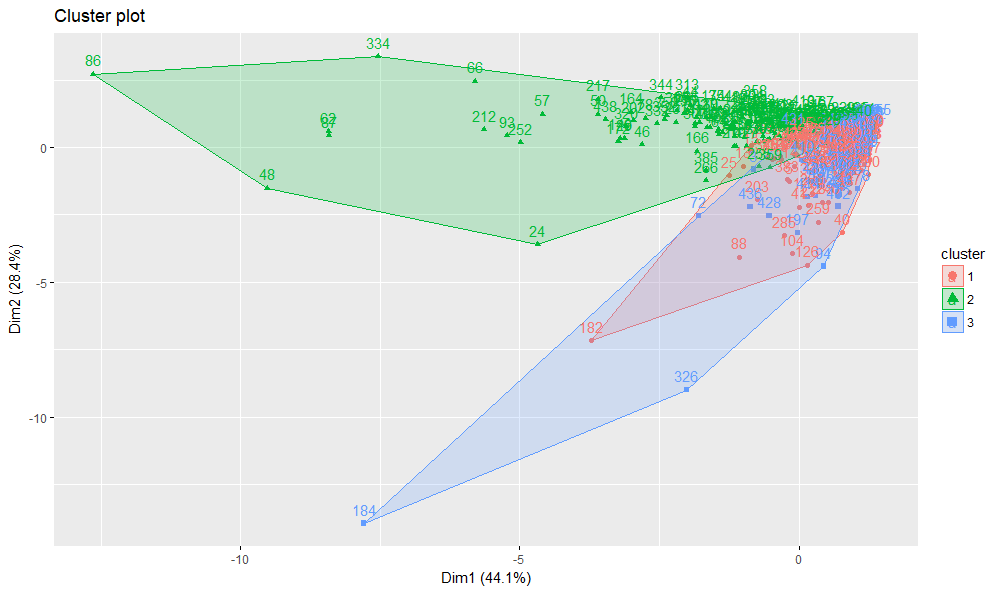
\includegraphics[scale=0.6]{clust}
\caption{Cluster Plot for the clusters obtained.}
\label{clustplot}
\end{figure}




%Beginning References. Don't add any text beyond this.
%------------------------------------------

\newpage %sending References to the last page

\bibliography{paper}
\bibliographystyle{apalike}
\end {document}